Šio magistro baigiamojo darbo tyrimams naudojami duomenys, kurie buvo naudoti darbų \cite{cnnExp1, cnnExp2} tyrimuose. Šių darbų tyrimuose naudoti duomenys yra laikomi repozitorijoje \cite{dataRepo}. Šioje repozitorijoje yra 1279115 3D modelių iš 662 kategorijų. Tačiau darbų \cite{cnnExp1, cnnExp2} tyrimuose yra naudojamas tik šių duomenų poaibis, kuris buvo sudarytas tyrimams atliktiems darbe \cite{dbnExp}. Šiame poaibyje yra 12311 3D modelių iš 40 kategorijų.

Kiekvienai kategorijai priklauso skirtingas skaičius modelių. Iš kiekvieno modelio darbe \cite{cnnExp2} yra sugeneruojama 12 2D nuotraukų. Visų nuotraukų kampai sudaro radialinę simetriją. Kitaip tariant, tarp dviejų kaimyninių pozicijų iš kurių buvo padaryta nuotrauka yra $30^{\circ}$ kampas iš objekto pozicijos. Visų nuotraukų pozicijos yra pakeltos $30^{\circ}$ kampu nuo horizontalės iš objekto pozicijos. Skirtingai negu darbo \cite{dbnExp} tyrimuose, darbo \cite{cnnExp2} tyrimuose nuotraukos yra generuojamos su juodu fonu ir kiekviena nuotrauka yra objektą apibrėžiantis stačiakampis (angl. bounding box). Kiekvienos nuotraukos matmenys yra $224\times224$. Šių duomenų pavyzdys yra pavaizduotas \ref{img:data_example} paveikslėlyje


\begin{figure}[H]
	\centering
	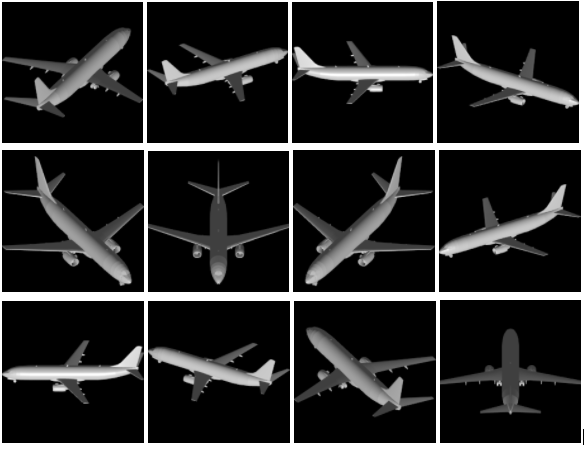
\includegraphics[scale=0.5]{img/data_example.png}
	\caption{Duomenų iliustracinis pavyzdys}
	\label{img:data_example}
\end{figure}

Darbų \cite{cnnExp1, cnnExp2} tyrimuose duomenys yra padalinami taip pat kaip darbo \cite{dbnExp} tyrimuose naudojami duomenys. Tad darbuose \cite{cnnExp1, cnnExp2, dbnExp} apmokymo aibė susideda iš 9843 modelių ir testavimo aibė -- 2468. Tačiau šiame magistro baigiamajame darbe, dėl kapsulinių neuroninių tinklų įgyvendinimo ypatumų yra apmokymui yra naudojama 9840 ir testavimui -- 2464.
